\label{Softwaremplementierung}

Für die entgültige Struktur der Software waren mehrere Anforderungen ausschlaggebend. \\
Zunähst wird beim Anschalten des Arduinos das Setup durchlaufen. Hier wird das \ac{LCD}-Display, angeschaltet und initialisiert. Dazu muss die Bibliothek <LiquidCrystal.h> eingebunden werden. Auch die Ein- und Ausgänge am Arduino wie Taster und \ac{LED}s werden hier definiert. Zudem geprüft, ob mit dem Mikro-SD-Karten-Adapter und CO$_2$-Sensor kommuniziert werden kann. \\
Falls der CO$_2$-Sensor nicht bereit sein sollte, wird eine Fehlermeldung ausgegeben. Nach erfolgreichem Start ist der Arduino angehalten so lange mit dem Starten des Programms zu warten, bis der Sensor zurückmeldet, dass er bereit ist, die Messung zu beginnen. \\
Aufgrund der Tatsache, dass wir den Sleep-Mode über eine Interrupt-Funktion erreichen, wird an dieser Stelle, mithilfe des Befehls <attachInterrupt()>, wie in Abbildung \ref{fig:InterruptDekl} zu sehen ist, die Funktion deklariert. \\
\begin{figure}[!hbt]
	\centering
	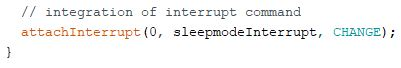
\includegraphics[width=0.6\linewidth]{Images/InterruptDekl}
	\footnotesize \\Quelle: eigene Aufnahme
	\caption{Codeausschnitt aus dem Setup zur Deklaration der Interrupt-Funktion}
	\label{fig:InterruptDekl}
\end{figure}
Anschließend befindet sich der Arduino softwaretechnisch im Loop, einer Endlosschleife. Hier werden zu Beginn jedes Durchlaufs alle \ac{LED}s ausgeschaltet. Ebenfalls wird der Cursor des \ac{LCD}-Displays auf die erste Stelle zurückgesetzt. \\
Zu Beginn des Programmablaufs wird der Anwender gefragt, ob er eine neue Messung starten, oder lieber die Letzte auslesen möchte. Ist das Auslesen der letzten Messung gewünscht, erleuchten die LEDs grün, gelb und rot. Dies soll dem Anwender die Bestätigung geben, dass die letzte Messung ausgelesen werden kann. Softwaretechnisch passiert an dieser Stelle nichts weiter, als dass der Arduino auf die Betätigung des Enter-Buttons wartet. Diese Auswahl hat den alleinigen Zweck, dass der Benutzer die Mikro-SD-Karte nicht während einer Messung entfernt und somit einen Fehler provoziert. \\
Falls der Anwender dennoch gegen die Vorgaben der Entwickler handeln sollte und die Mikro-SD-Karte während einer Messung herausnimmt, wird diese trotzdem bis zum Ende durchgeführt. Die resultierende Konsequenz ist, dass sich auf der Mikro-SD-Karte keine Datei befindet, da der Mikrocomputer nicht die Möglichkeit hatte die angelegte Text-Datei abzuspeichern. \\
Handelt der Anwender im Sinne der Entwickler und wählt zum Entfernen der Mikro-SD-Karte den Lese-Modus, kann er nachdem diese wieder im Adapter ihren Platz gefunden hat, den Vorgang mit dem Enter-Button bestätigen. So öffnet sich wieder das Hauptmenü und eine neue Messung kann auf Wunsch gestartet werden. \\
Als nächstes wurden drei verschiedene Messprofile definiert und implementiert, sodass der Benutzer zwischen einer Echtzeit-, Stunden- und Tagesmessung wählen kann. In diesen Messprofilen ist definiert, in welchen Abständen und wie lange Messungen durchgeführt werden sollen. Somit konnten Anforderung Nummer 1 und 10 aus der Tabelle \ref{tab:Anforderungen} gemeinsam umgesetzt werden. Diese Messmodi sind global mithilfe des Befehls <\# define> festgelegt. \\
Nach der Wahl des Messprofils muss der Arduino den CO\textsubscript{2}-Sensor ansteuern und richtig konfigurieren. Es muss getestet werden, ob er funktionstüchtig und bereit ist, eine Messung zu starten. Dies konnte durch eine if-Bedingung abgefragt werden. \\
Zudem kann der verwendete Sensor nicht nur CO\textsubscript{2}-Werte, sondern beispielsweise auch Temperaturen messen, sodass der Arduino die richtigen Werte anfordern muss. Damit dies möglich ist, musste die Bibliothek <Adafruit\_CCS811.h> eingebunden werden. Genaueres zu dem Algorithmus dieser Bibliothek wird in Kapitel \ref{CCS811} erläutert. \\
Auch während dem Programmdurchlauf wird bei jeder neuen Messung kontrolliert, ob der CO\textsubscript{2}-Sensor funktionstüchtig ist. Danach wird mithilfe der oben genannten Bibliothek der CO\textsubscript{2}-Wert gemessen und an den Arduino weitergegeben. \\
Nach Einlesen der Daten, vergleicht der Mikrocomputer diese mit den gegebenen Grenzwerten. Je nach Bewertung des gemessenen Wertes wird eine der grün, gelb oder roten \ac{LED}s eingeschaltet. Auch die blaue \ac{LED}, welche die Ansteuerung des automatisierten Fensterscheibenmotors simulieren soll, wird je nach Messwert an- oder ausgeschaltet. Zudem werden dem Anwender die jeweiligen Daten im \ac{LCD}-Display ausgegeben. \\
Damit der Verlauf der Messung später auf Excel geplottet werden kann, wird der gemessene Wert im .csv-Format auf einer Mikro-SD-Karte als .txt-Datei abgespeichert. Das bedeutet, dass die Messungen in einer Zeile, getrennt durch Kommas, gesichert werden. Dies wird durch den Befehl <textfile.print()> ermöglicht. \\
Falls Excel trotzdem alle Werte in ein Feld schreiben sollte, anstatt jeden Wert in einem solchen Feld anzuzeigen, kann dieses Problem innerhalb von Excel berichtigt werden. In der Menüleiste von Excel muss das Feld <Daten> ausgewählt werden. Durch die Markierung des Eintrags und Auswählen des Feldes <Text in Spalten>, können die Trennzeichen händisch definiert werden. Nachdem Kommas als Trennzeichen ausgewählt wurden, teilen sich die Messungen in Spalten auf. Nun kann, durch Markierung aller Messwerte und der Auswahl des gewünschten Diagramms, der Verlauf der Messung dargestellt werden. \\
Nachdem der letzte Wert auf der Mikro-SD-Karte gespeichert wurde, beginnt das Programm durch die Anzeige des Hauptmenüs, automatisch von vorne. Falls der Sleep-Mode-Button während des Programmablaufs gedrückt wurde, springt das Programm in einen Art Stromspar- oder auch Schlafmodus. Hier gehen sowohl alle Lampen, als auch die Beleuchtung des \ac{LCD}-Displays aus. Wie am Anfang des Kapitels erwähnt, wurde dieser Taster als Interrupt implementiert. Es muss somit nicht ein weiteres Menü kreiert werden, um den Anwender zu fragen, ob dieser den Sleep-Mode aktivieren möchte. Das ermöglicht dem Anwender, den Sleep-Mode-Button zu jedem beliebigen Zeitpunkt zu betätigen. Dem Benutzer ist garantiert, dass der Arduino, nach Beenden der aktuellen Messung, in den Schlafmodus geht. \\
Das Wieder-Aufwecken der Hardware geschieht durch eine Betätigung des Enter-Buttons. Das Betätigen eines anderen Tasters wird ignoriert. Auch das wiederholte Drücken des Sleep-Mode-Buttons soll nicht von Relevanz sein, damit der Anwender später den Enter-Button nicht öfter drücken muss, da der Schlafmodus mehrere Ebenen kreiert. \\
Damit dies gewährleistet ist, setzt die Interrupt-Funktion, welche in Abbildung \ref{fig:InterruptFunktion} zu sehen ist, eine Variable auf den Wert Eins. \\
\begin{figure}[!hbt]
	\centering
	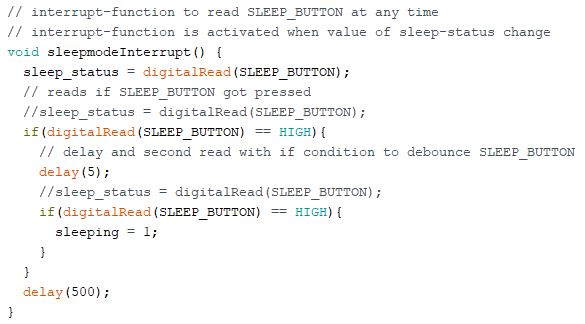
\includegraphics[width=0.8\linewidth]{Images/InterruptFunktion}
	\footnotesize \\Quelle: eigene Aufnahme
	\caption{Codeausschnitt: ausgelagerte Interrupt-Funktion mit Tastenentprellung, für das Werten der Variable, zur späteren Aktivierung des Schlafmodus}
	\label{fig:InterruptFunktion}
\end{figure}
\newpage
Solange die Variable den Wert Eins beibehält, bleibt der Arduino in seinem Schlafmodus. Bei Betätigung des Enter-Buttons wird diese Variable wieder auf Null zurückgesetzt und das Programm kann fortgeführt werden. Die Softwareimplementierung ist in Abbildung \ref{fig:InterruptAktivierung} zu sehen. Wird der Sleep-Button also öfter gedrückt wird der Wert dieser Variablen immer wieder auf Eins gesetzt, was den Zustand des Arduinos nicht verändert. \\
\begin{figure}[!htb]
	\centering
	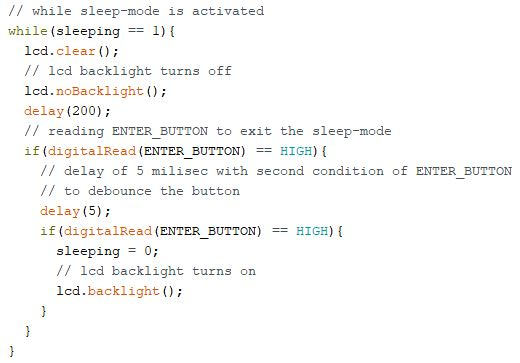
\includegraphics[width=0.7\linewidth]{Images/InterruptAktivierung}
	\footnotesize \\Quelle: eigene Aufnahme
	\caption{Codeausschnitt aus dem Loop zur Aktivierung und Deaktivierung des Schlafmodus}
	\label{fig:InterruptAktivierung}
\end{figure}
\newline
Nach Verlassen des Sleep-Modes, durch die Betätigung des Enter-Buttons, erscheint wieder das Hauptmenü. Das Programm kann nun erneut von vorne gestartet werden. 